The implementation of  PyGromosTools tries to accomplish several goals that were identified to be crucial for good API development: \cite{Henning2009, Blanchette2008, Bloch2006}
\begin{itemize}
    \item An API is easy to learn and memorize, such that coding with it comes naturally. 
    \item The usage of an API should lead to better readable code.
    \item A well-designed API is hard to misuse and easy to extend.
    \item Last but not least, an API is complete and simple. However, this can develop over time.
    \item Design an API with context knowledge for the field of usage. 
\end{itemize}

As PyGromosTools is a package that needs to deal with the history of GROMOS and has a non-linear history, it needs to balance the amount of technical debt and the progress in projects very well. However, the package slowly converges to a consistent form. By now we believe, that the general structure of usage is established with long-term sustainability.
The rigidification of specific usage patterns on the user level is vital to sustaining a long-term experience that does not crash old code.  

If all criteria are fulfilled, the easy-to-use, reproducible, fast, expandable simulation setup and execution of molecular dynamics simulations will lead to a higher quality of scientific output in terms of openness, accessibility, and reproducibility.

\subsection{Coding Paradigms}
PyGromosTools follows several modern Coding styles. These are not enforced on users, but the style is enforced on PyGromosTools developers who would like to contribute. 

%code visibility/information hiding
Information hiding is an essential concept in coding for larger projects. It boils down to presenting only the required information to a reader. Usually, larger packages have thousands of lines of code, and presenting all of them at the same time gets very overwhelming. Therefore encapsulation of code into functions and classes or managing the accessibility of certain variables/functions is hugely important in code hiding. \cite{} 

In PyGromosTools, accessibility is managed with the provided methods by python. For example are private variables in the \textit{GROMOS\_System} assigned with a prefix "\_" like the attribute \textit{\_GROMOSPP} (see  \hyperlink{https://github.com/rinikerlab/PyGromosTools/blob/348439a326357b8172717f5d5ed7a5bbfa4564ab/pyGROMOS/files/GROMOS\_system/GROMOS\_system.py\#L83}{Code}). Note that this way of declaring a variable still  makes it easily accessible in practice. If a variable of function should clearly never be used externally name mangling is used with the prefix "\_\_" like \textit{\_\_ionDecorator} (see  \hyperlink{https://github.com/rinikerlab/PyGromosTools/blob/348439a326357b8172717f5d5ed7a5bbfa4564ab/pyGROMOS/files/GROMOS\_system/GROMOS\_system.py\#L994}{Code}) like defined in \hyperlink{https://www.python.org/dev/peps/pep-0008/}{PEP 8}.
The second aspect of encapsulation of code into functions and classes is the modularization of the code. This concept allows quick construction of more complex structures and therefore speeds up the development process and readability at the same time. \cite{}

\subsubsection{Variables, Signatures, and Classes}
PyGromosTools, in general, follows the principle of using descriptive variables. Each naming in the package should give a comprehensive description of the function of a definition. Abbreviations are therefore forbidden. Following this paradigm increases the general readability of the code, leading to a clearer understanding of code and, therefore, avoiding mistakes. 
Consequentially, the second style decision for PyGromosTools is annotating types of variables in classes and functions and function return types. This style follows the python enhancement proposals  \hyperlink{https://www.python.org/dev/peps/pep-0526/}{PEP 526}, \hyperlink{https://www.python.org/dev/peps/pep-0484//}{PEP 484} , and  \hyperlink{https://www.python.org/dev/peps/pep-3107/}{PEP 3107} which implemented the type annotation system of python3. This decision was made because of the more complex types in PyGromoTools, in order to provide quick tips to users and developers on which type is the expected type. The type annotations can be quickly accessed in the source code, are visualized in IDEs or interactive python sessions. 
A third style choice is the usage of keyword arguments used in function parameter passing. The keyword argument passing was introduced with \hyperlink{https://www.python.org/dev/peps/pep-0468/}{PEP468} the underlying reason for the usage of this feature is the increased readability of the code and making the code more robust versus code refactoring of function signatures.

\subsection{Documentation and Continous Integration}
In PyGromosTools, each function and module should contain a docstring description. The chosen docstring style is \hyperlink{https://numpydoc.readthedocs.io/en/latest/format.html}{numpydoc} from the NumPy package. \cite{VanDerWalt2011} The doc-string style is supported over various IDEs and is automatically collected in the documentation via sphinx.
Additionally to the documentation are several jupyter-notebooks provided exemplifying the usage of PyGromosTools on multiple layers. \cite{Kluyver2016}
Besides this, a continuous integration pipeline is implemented with a set of unit tests that ensure the base functionality of the package.


\subsection{Object Oriented and Functional Programming}
Python3 is a multi-paradigm language allowing for mixing OOP and functional programming styles. Generally, PyGromosTools focuses on OOP. 

On the one hand, OOP brings the benefits of inheritance the subsequent concept of polymorphism. These concepts are used in PyGromosTools with state-driven contexts like file representations or the submission system classes. Especially in the base class \textit{\_general\_GROMOS\_file} contains the, for example, the fundamental read/write procedures, that are the same for all GROMOS files and therefore is only implemented once. (see \hyperlink{https://github.com/rinikerlab/PyGromosTools/blob/348439a326357b8172717f5d5ed7a5bbfa4564ab/pyGROMOS/files/\_basics/\_general\_GROMOS\_file.py\#L15}{Code})

On the other hand, functional programming can be found in subsequent function implementations, realized with, for example, map, apply, and zip operations, or even as higher-level functional programming with python decorators. As an example for the Decorators, the principle of currying was realized for the GROMOSPP integration into the GROMOS system, such as the dynamically generated functions update the attribute files of the GROMOS system automatically, and those do not need to be provided to the function call (see Figure \ref{fig: GROMOSSystemSimulationExample}) (see  \hyperlink{https://github.com/rinikerlab/PyGromosTools/blob/348439a326357b8172717f5d5ed7a5bbfa4564ab/pyGROMOS/files/GROMOS\_system/GROMOS\_system.py\#L915}{code}). \cite{Curry1958}


\subsection{Code Structure}
PyGromosTools itself has two layers. 
The lowest layer is building interfaces/APIs to establish communication with the operating system, the queueing system, or the GROMOS wrappers. All these functions are used in the next layer to build more complex structures that fulfill more complex tasks. 

In the following, we want to discuss the implementation of the different modules of PyGromosTools. In general, one can split the package into four modules: Data, Files, Simulation, Analysis.  


%The fundamental idea of files
The file module is a collection of classes that represent the different GROMOS-files in python. The module's design is based on the object-oriented programming paradigm (OOP) and therefore makes extensive use of inheritance and polymorphism to build up a class structure in the sense of the GROMOS File structure with a minimal amount of code duplications.
In the GROMOS file structure, each file contains multiple blocks. These blocks contain either a table of data or a  list of values. The structure of files in PyGromosTools is compatible with this structure and makes the experience pattern similar to the design of GROMOS. The structural fundament is placed in the \textit{\_general\_GROMOS\_file} class that was created to contain fundamental functionality that is encoded in the general file structure. Resulting functions are \textit{read\_file}, \textit{write} or \textit{str}-operator overloading.
This generic file class encapsulates classes derived from \textit{\_generic\_GROMOS\_blocks} which again provides generic functions like read-  and write-functionalities as well as overloading operators. 
The most elementary structure is the one used by the generic blocks as content. This structure is in many blocks the \textit{\_generic\_field}, a direct primitive type or a pandas data frame. (see Figure \ref{subFig-GeneralFileGROMOSXX})

%Features
All these compartments generate specific classes for the different files used in the GROMOS environment. Features of these classes are: 
\begin{itemize}
    \item IO functionalities that not only allow writing files but also writing obj states or converting files.
    \item The direct accessibility of any type of GROMOS data in the objects allows a lean integration into python3 scripts.
    \item Additional functionality, that directly works on the file class like: calculating trajectory RMS or removing residues from \textit{CNF}s.
\end{itemize}

% generation of coordinates/atoms/molecules and topology generation of topology terms with correctness checking (is bond already present, etc. ) wrappers for simulation parameter blocks


%File Types
From the GROMOS environment, most files were implemented in PyGromosTools with an individually class derived from the \textit{\_general\_GROMOS\_file} class and sorted into the different categories of their functionality.
The class realizations span over aspects of the MD-Package, like coordinate files, topologies, simulation parameter files, trajectories, forcefield files, and other files like replica-exchange outputs or NMR GROMOSPP program output files. The Force Field Class ForceField System represents a whole forcefield in this environment and allows the capability of parametrizing molecules. (see Figure \label{subFig-FilesinModule})

The trajectory files translate the GROMOS trajectory in a pandas data frame that can quickly and efficiently be used on the python. The data frame is stored in the compressed hf5 format and, therefore, is very storage efficient.
%Todo: MTB files / lib files oder so trf, trs, trv

%%GROMOS System
All the different file formats can be stored centralized in the GROMOS System class. This class is the central structure of PyGromosTools, from which any simulation approach can be started. The class can be used with a minimal set of files, like coordinate file (.cnf), topology file (.top), and a simulation parameter file (.imd) or even just with a molecule SMILE/RDKit Mol string which leads to a complete parametrization with openFF.

% off

%% helper functions that adapt system, future flag, auto convert (oFF topo,conv, adaptIMD from smiles)
%%interface forcefield SYS

%conc Outlook
Due to the consequent inheritance structure, new blocks or files can be implemented very easily and quickly. 
In theory, this API could also introduce new file types that are easier to handle without omitting the old ones. For example, the Simulation parameters file could easily be translated into a JSON or XML data format, making the file handling and readability through the key-value policy much more accessible.

\begin{figure}[h]
    \centering
    \begin{subfigure}{1\textwidth}
        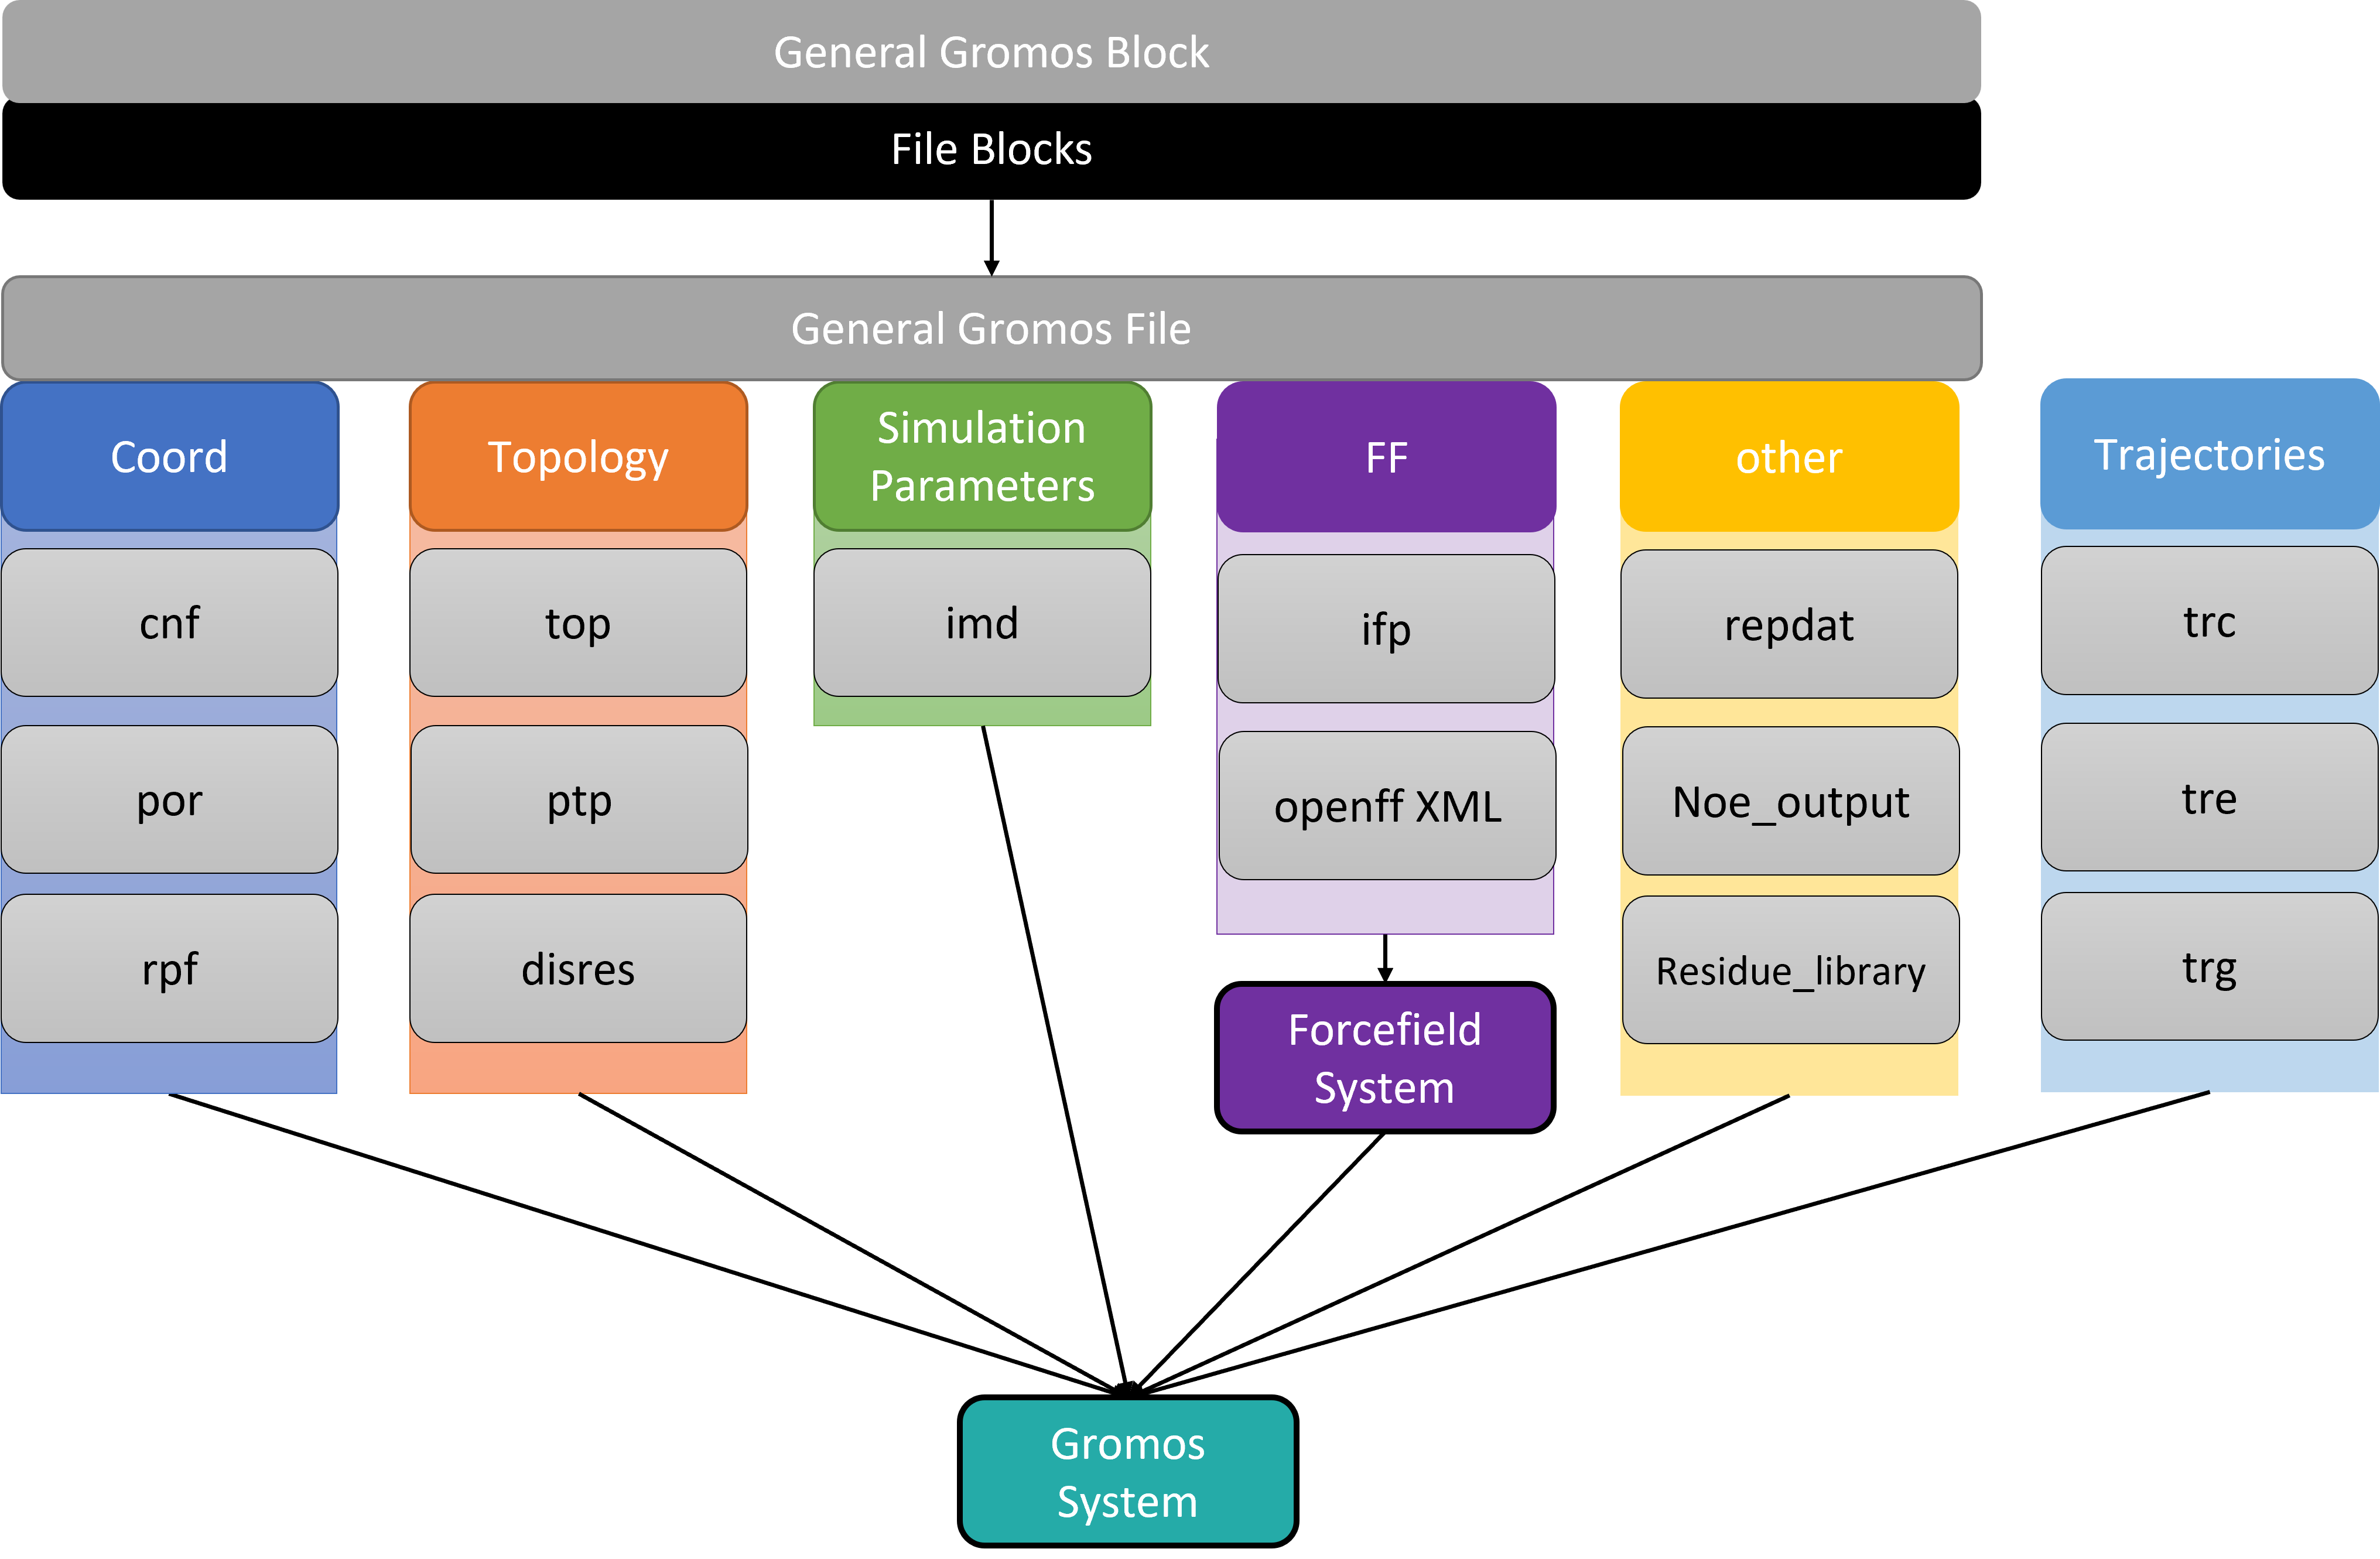
\includegraphics[width=\textwidth]{fig/implementation/Files.png} 
        \caption{}
        \label{subFig: FilesinModule}
    \end{subfigure}
    \caption{Files Module:  The PyGROMOS module Files is implemented with an OOP structure based on the GROMOS file structure. The base classes are the \textit{\_generic\_GROMOS\_block} and the \textit{\_general\_GROMOS\_file}. From these base classes all the different GROMOS blocks and GROMOS files are derived, with the exception of trajectories, in order to provide a consistent experience.
    In the figure only the implemented file classes are shown for clarity. As a central element of PyGromosTools, the GROMOSSystem class collects all files and makes them easily accessible for simulation approaches or other functionality that requires multiple GROMOS files.
    }
    \label{fig: FileModule}
\end{figure}

\subsection{Simulation Module}
The module simulations contain multiple submodules used to realize GROMOS simulations, ready for HPC-Queueing on different hardware setups. The submodules of simulations can be arranged into three layers. This structure allows fast adaptation of functionality in these modules (see Figure \ref{fig: SimulationModule}).

One foundation of this module is the two submodules GROMOS and HPC-Queuing. GROMOS contains the python API to the GROMOSXX and GROMOSPP C++ code, allowing quick access to their functionality. Currently is the API of GROMOSXX and GROMOSPP realized in the form of bash wrappers that provide the functionality. Nevertheless, we believe that proper C++ python integration would be beneficial to improve the communication between the layers. Recently a pyGROMOSPP compartment was added that contains efficient python implementations of several functionalities similar to the style of GROMOSPP. In general, we believe that the advantages of the python language and the possibility of writing more efficient code with modern python packages will lead to a growth of GROMOSPP functionality implemented directly into the python layer instead of a more complicated C++ implementation. The GROMOS module can be used isolated from all other modules to allow fast development in other parts of the packages or for specific projects.

The second foundation of this module is the HPC-Queuing module. It builds an interface to job-management tools like LSF and provides the functionality of job queueing for PyGromosTools scripts. The submodule is divided into a submission system and a job scheduling part. The submission system part is structured into an OOP-based structure with the parent class \textit{\_SubmissionSystem} that functions as an interface, ensuring the correct implementation of the child classes. Already implemented submission system classes are: 
\textit{DUMMY}, a class that only prints out strings, and therefore can be easily used for testing. \textit{LOCAL}, this class is executing every submitted job directly on the local machine via the operating system. Last, the class \textit{LSF} for the IBM Queueing system. This class allows the scheduling of simulations on the HPC cluster using the LSF queuing system. The class was optimized for the Euler cluster.
Besides the submission systems, the HPC-Module contains job scheduling tools that implement a scheduler worker pattern (see Figure \ref{fig: SimulationExecPattern}). In this pattern, a scheduler function submits worker sub-scripts dynamically generated from template workers to the queueing system, effectively executing the submitted steps in order. Present workers are the simulation, the clean-up, and the analysis worker. The separation of these three tasks is essential for guaranteeing the correct execution of the different tasks.

A good usage pattern for the submission systems is starting to develop a pipeline with the DUMMY or LOCAL submission system locally and then upscale the approach to the HPC-Cluster. This pattern proved to be a practical and straightforward approach as many problems/bugs can be already caught locally without wasting time queueing and stressing the Cluster with traffic.

\begin{figure}[h]
    \centering
    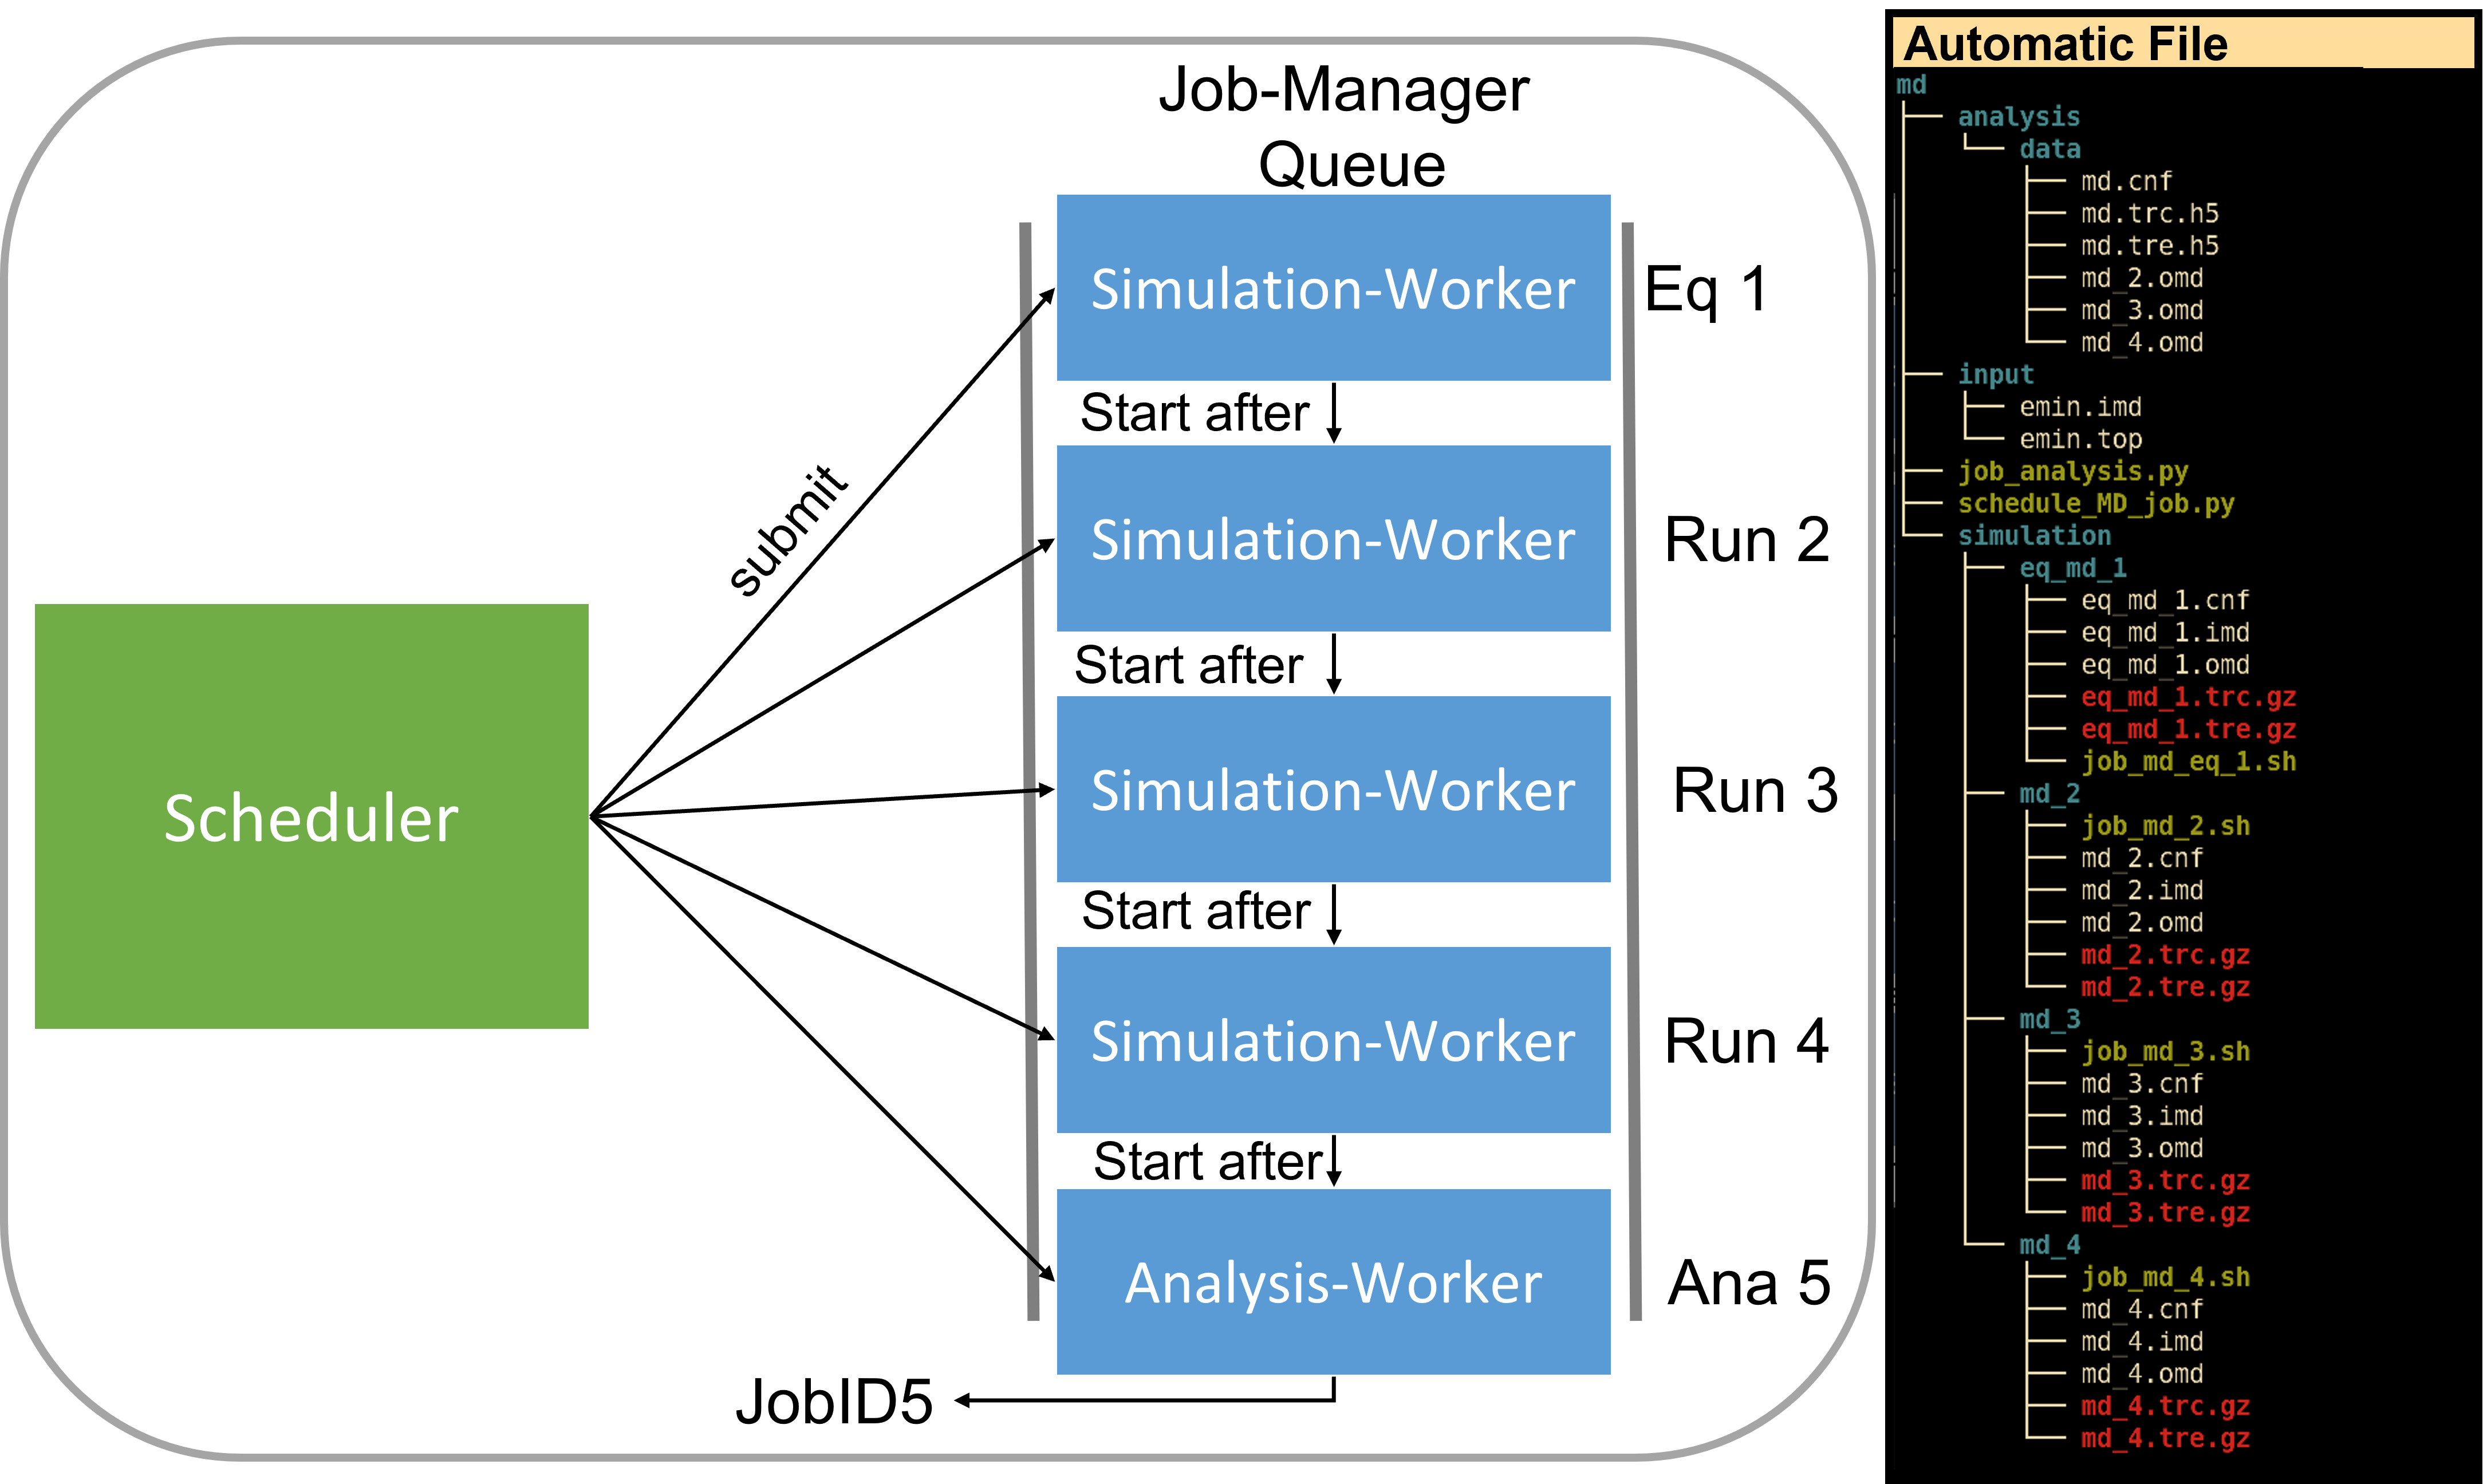
\includegraphics[width=\textwidth]{fig/implementation/SimulationExecutionManagment.png}
    \caption{HPC-queuing submission pattern: The implemented submission pattern of the HPC-Queuing module follows the pattern of using a scheduler function, that submits worker scripts that perform the whole work or a part of it.The worker script is directly executed or submitted to a job-manager tool based on the provided submission system class. The automatically generated file structure by the exemplified execution is shown in the right box. Note that the simulation directory is compressed in the process. The md folder was uncompressed in the figure to illustrate the concept.Generally, the user can delete this compressed folder, but it is only advised after finishing a project. The code for this example is shown in Figure \ref{fig: GROMOSSystemSimulationHPCExample}. }
    \label{fig: SimulationExecPattern}
\end{figure}

The two described submodules are combined in the simulation blocks, which can directly execute simulations. As required input, the simulation blocks take only a GROMOS system, which contains all input files. If no IMD file is provided, a template file for the simulation approach will be mapped on the system. By exchanging the default submission system (\textit{LOCAL}), the described upscaling can be performed easily. Besides automatic scheduling of tasks, the function also provides automatic file management for the simulation (see Figure \ref{fig: SimulationExecPattern}). The output of the simulation function is a copy of the input simulation adapted to contain the output files of the simulation. If the simulation was directly executed, these files are directly parsed into the class. However, if the simulation is queued, all the non-present output files are marked with an \textit{\_future} flag. This flag prevents the system from executing tasks on the object that requires the presence of the data. In more complex simulation chaining approaches, these tagged files can be used to submit follow-up simulation steps (e.g., reeds s-optimization or Eoff-rebalancing approach). If a file is existent at a later time point, the \textit{\_future\_promise} flag is removed by the \textit{\_check\_promises} and the file is automatically loaded into the GROMOS system object.
Additional minor features are checking if simulations or analysis scripts were already finished successfully or if the current job was already submitted to the queue, all leading to skipping the step. And the final concatenation of files and storing as compressed .h5 PyGromosTools-trajectory files in analysis/data (see Figure \ref{fig: SimulationExecPattern}).

%Simulation Approaches
\begin{figure}[h]
    \centering
    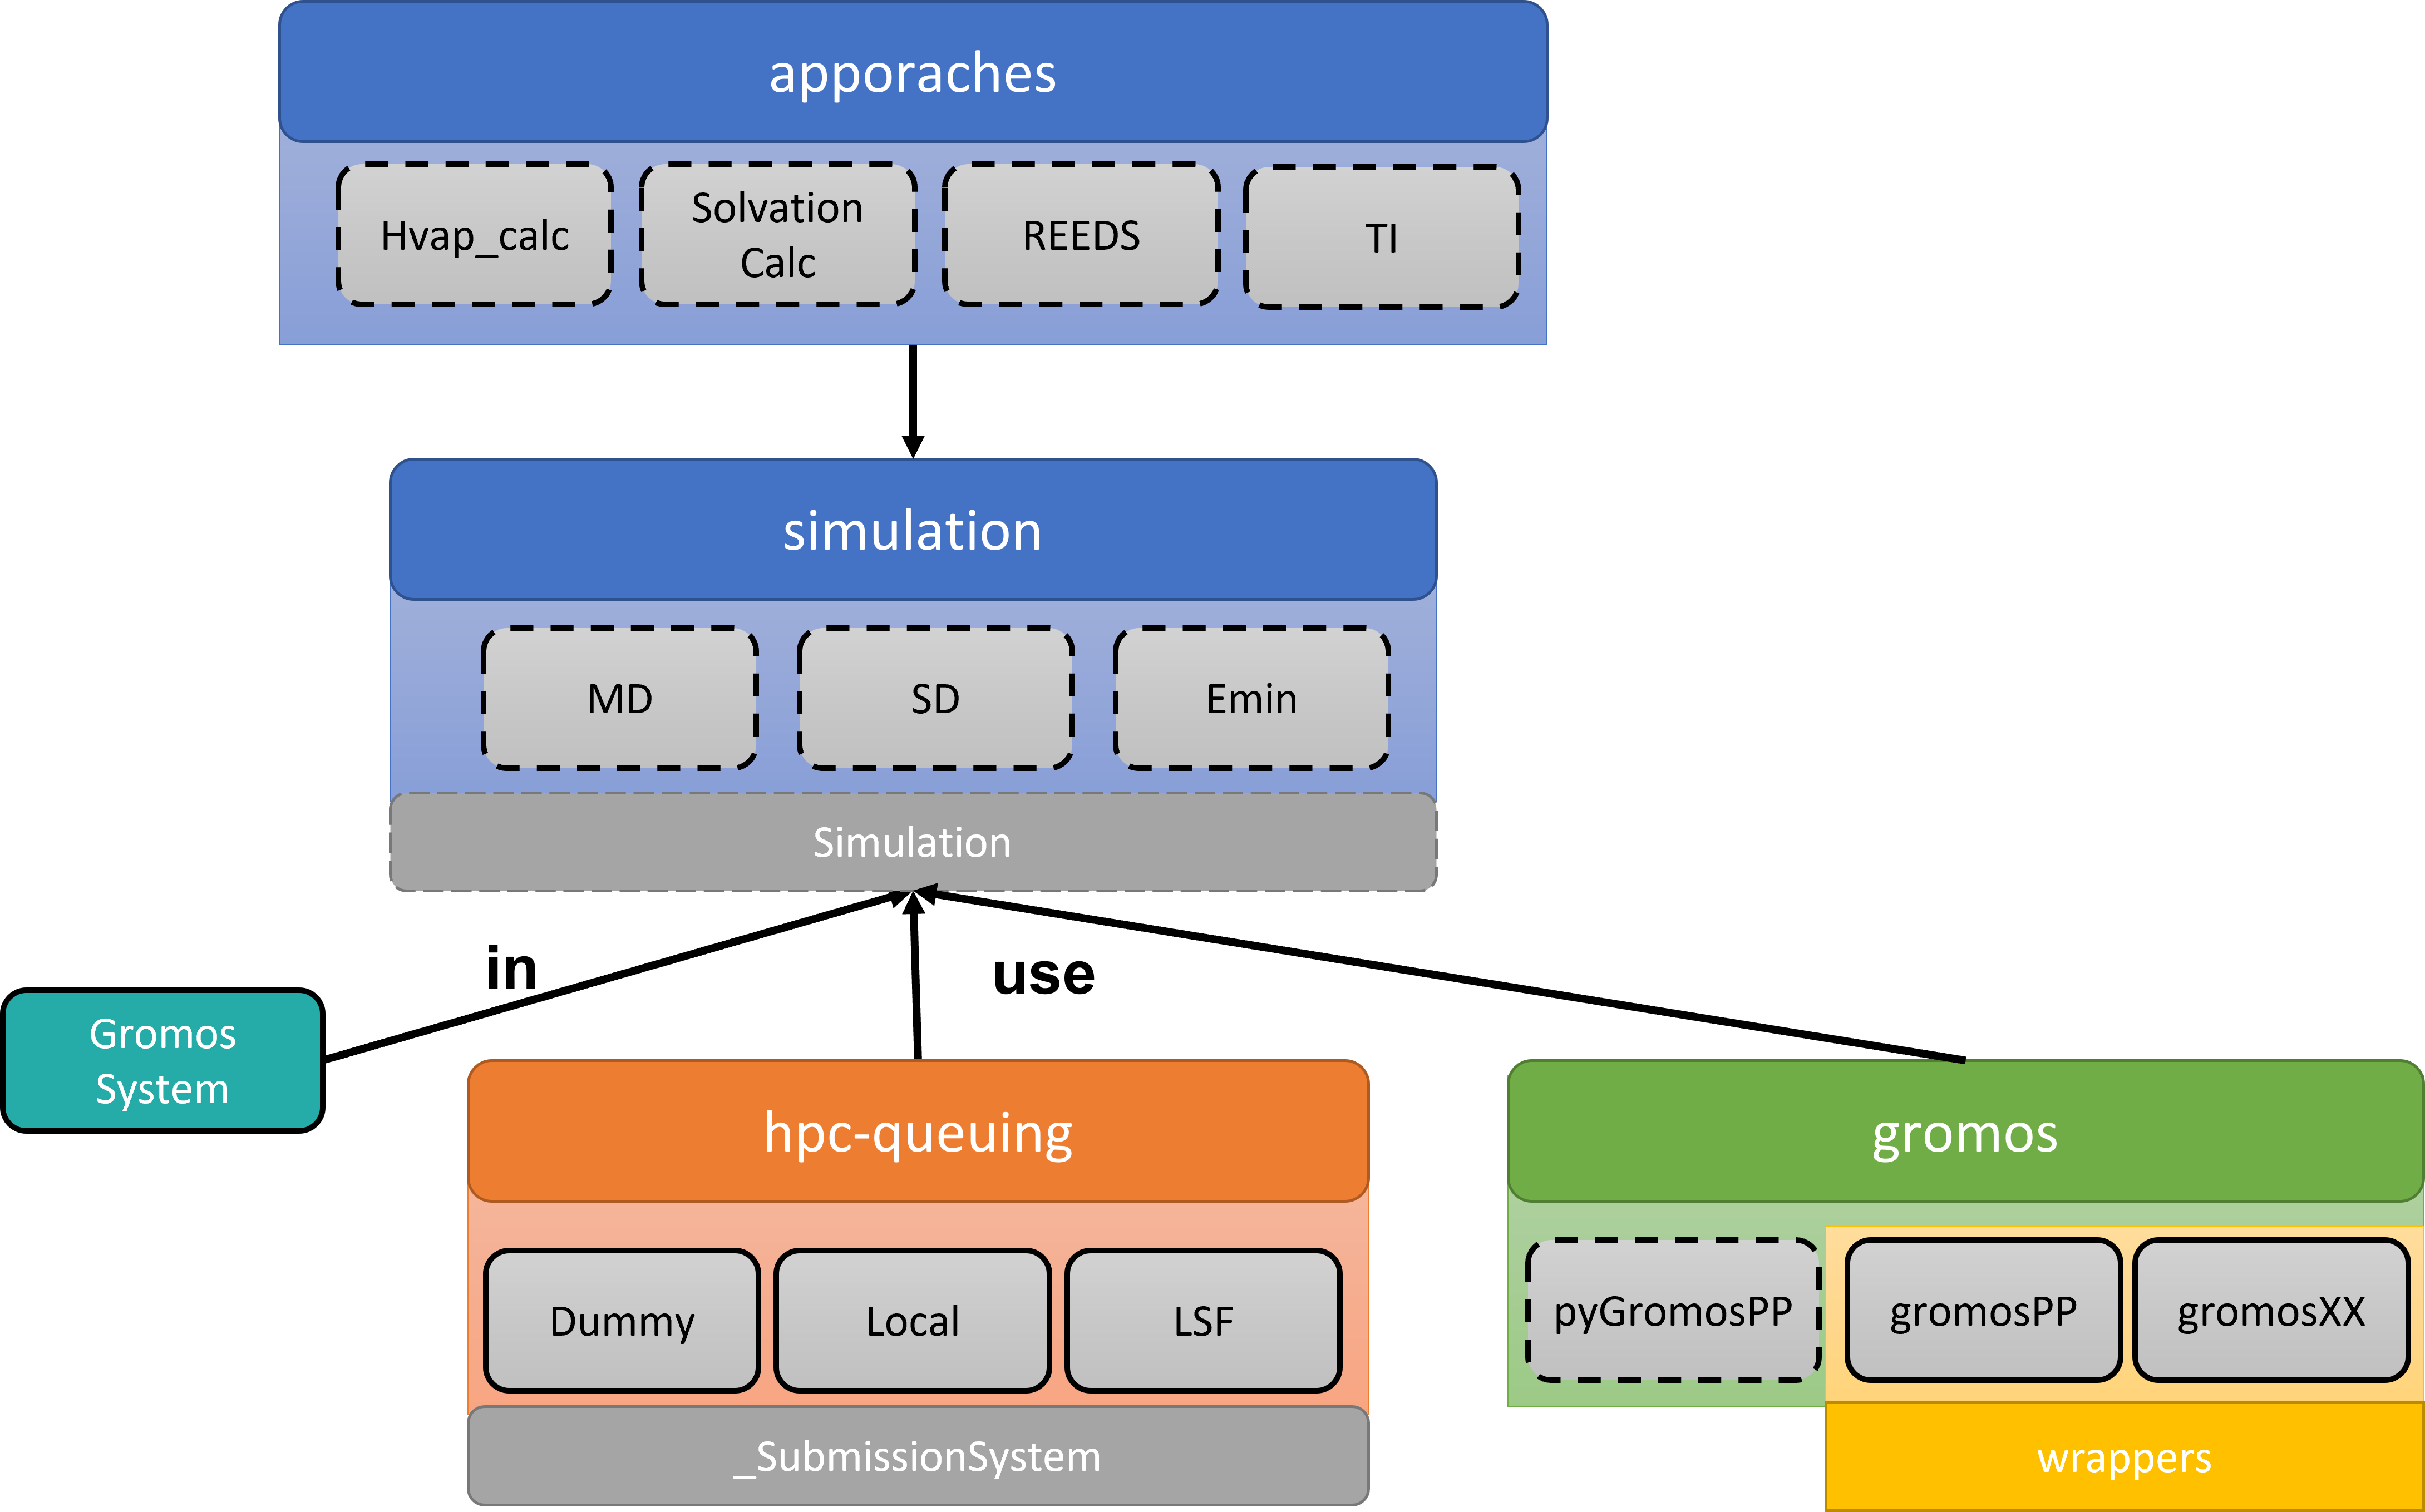
\includegraphics[width=\textwidth]{fig/implementation/Simulation.png}
    \caption{Simulation Module: The simulation module contains two submodules, HPC-queuing and GROMOS. GROMOS is the API to all GROMOS functionality written in C++ and a new module containing GROMOSPP like functionality in python. The HPC-queueing Submission System classes can be used to adapt a simulation approach to a different environment quickly  (e.g., local execution or queuing with the LSF-Job management tool on the Euler cluster). This adaptation is possible due to the commonly shared parent class \textit{\_SubmissionSystem}. The simulation module provides functions that wrap HPC-queuing and GROMOS functionality providing quick access to performing GROMOS Simulations. Additionally are higher-level approaches present that can be used for simulating. Here dashed box borders imply based on functions, and bold box borders imply an underlying class structure.}
    \label{fig: SimulationModule}
\end{figure}

The final compartment of the simulations module is the approaches directory. In this submodule, high-level approaches are stored that fulfill a complete simulation approach, like calculating free energies for evaporation or thermodynamic integration simulations (used for Restraintmaker).

\subsection{Analysis \& Module}
The analysis module contains functionality for analyzing and visualizing properties and structures. The analysis functions can calculate properties over trajectories like estimating free energies, calculating coordinate RMSDs, and more. The visualization tools use py3dmol and enable visualization of coordinate files or trajectories in jupyter notebooks. The analysis package is the youngest module of PyGromosTools and will grow in the future. As a bonus, the data module provides the package with parameters for force fields like the GROMOS 54A7 force field and template simulation parameter files to have a good start for a simulation (see Figure \ref{fig: GROMOSSystemExample} or \ref{fig: GROMOSSystemSimulationExample})
